\documentclass{article}
\usepackage[papersize={8.38cm,6.15cm},margin=0pt]{geometry}
\usepackage{tikz}
\usepackage{newtxtext,newtxmath}
\pagestyle{empty}
\parindent=0pt

% x(bucket i) = i*1.44 cm (i = 0..4) ; y(rate) = rate * 3.4 cm
\begin{document}
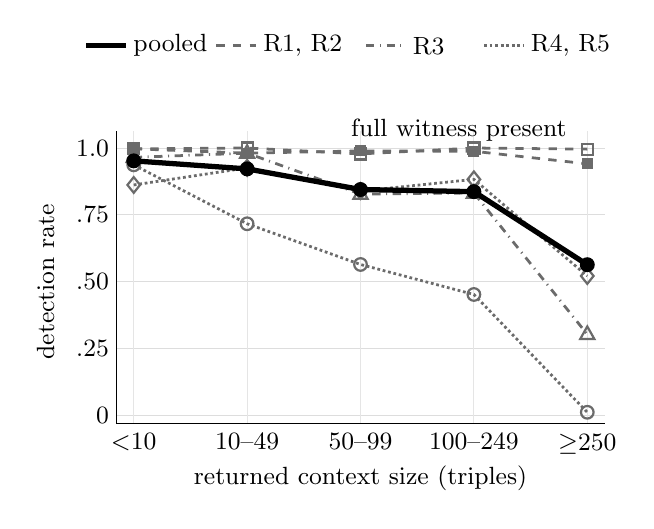
\begin{tikzpicture}[x=1cm,y=1cm]
\begin{scope}[shift={(1.22,1.02)}]

\foreach \y in {0,0.85,1.7,2.55,3.4}
  \draw[gray!27,line width=0.35pt] (-0.22,\y) -- (5.98,\y);
\foreach \i in {0,1,2,3,4}
  \draw[gray!20,line width=0.35pt] (\i*1.44,-0.1) -- (\i*1.44,3.62);
\draw[line width=0.6pt] (-0.22,-0.1) -- (-0.22,3.62);
\draw[line width=0.6pt] (-0.22,-0.1) -- (5.98,-0.1);

\foreach \y/\l in {0/0,0.85/{.25},1.7/{.50},2.55/{.75},3.4/{1.0}}
  \node[left,font=\small,inner sep=2.5pt] at (-0.22,\y) {\l};
\foreach \i/\l in {0/{$<$10},1/{10--49},2/{50--99},3/{100--249},4/{$\ge$250}}
  \node[below,font=\small,inner sep=3.5pt] at (\i*1.44,-0.1) {\l};
\node[font=\small] at (2.88,-0.80) {returned context size (triples)};
\node[rotate=90,font=\small] at (-1.12,1.7) {detection rate};

% R1  .997 1.000 .978 1.000 .996
\draw[black!58,dashed,line width=1.0pt] (0,3.390) -- (1.44,3.400) -- (2.88,3.325) -- (4.32,3.400) -- (5.76,3.386);
\foreach \i/\y in {0/3.390,1/3.400,2/3.325,3/3.400,4/3.386} \draw[black!58,line width=0.8pt] (\i*1.44-0.07,\y-0.07) rectangle (\i*1.44+0.07,\y+0.07);
% R2  .997 .981 .989 .988 .941
\draw[black!58,dashed,line width=1.0pt] (0,3.390) -- (1.44,3.335) -- (2.88,3.363) -- (4.32,3.359) -- (5.76,3.199);
\foreach \i/\y in {0/3.390,1/3.335,2/3.363,3/3.359,4/3.199} \fill[black!58] (\i*1.44-0.07,\y-0.07) rectangle (\i*1.44+0.07,\y+0.07);
% R3  .965 .981 .828 .832 .304
\draw[black!58,dash dot,line width=1.0pt] (0,3.281) -- (1.44,3.335) -- (2.88,2.815) -- (4.32,2.829) -- (5.76,1.034);
\foreach \i/\y in {0/3.281,1/3.335,2/2.815,3/2.829,4/1.034} \draw[black!58,line width=0.8pt] (\i*1.44,\y+0.10) -- (\i*1.44-0.09,\y-0.06) -- (\i*1.44+0.09,\y-0.06) -- cycle;
% R4  .862 .926 .839 .883 .522
\draw[black!58,densely dotted,line width=1.0pt] (0,2.931) -- (1.44,3.148) -- (2.88,2.853) -- (4.32,3.002) -- (5.76,1.775);
\foreach \i/\y in {0/2.931,1/3.148,2/2.853,3/3.002,4/1.775} \draw[black!58,line width=0.8pt] (\i*1.44,\y+0.10) -- (\i*1.44-0.08,\y) -- (\i*1.44,\y-0.10) -- (\i*1.44+0.08,\y) -- cycle;
% R5  .937 .717 .565 .453 .013
\draw[black!58,densely dotted,line width=1.0pt] (0,3.186) -- (1.44,2.438) -- (2.88,1.921) -- (4.32,1.540) -- (5.76,0.044);
\foreach \i/\y in {0/3.186,1/2.438,2/1.921,3/1.540,4/0.044} \draw[black!58,line width=0.8pt] (\i*1.44,\y) circle (0.08);
% pooled  .952 .922 .845 .837 .564
\draw[black,line width=1.9pt] (0,3.237) -- (1.44,3.135) -- (2.88,2.873) -- (4.32,2.846) -- (5.76,1.918);
\foreach \i/\y in {0/3.237,1/3.135,2/2.873,3/2.846,4/1.918} \fill[black] (\i*1.44,\y) circle (0.095);

\node[font=\small,anchor=east] at (5.62,3.62) {full witness present};
\end{scope}

% legend
\begin{scope}[shift={(0.62,5.72)}]
  \draw[black,line width=1.9pt] (0,0) -- (0.5,0);
  \node[right,font=\small,inner sep=2.5pt] at (0.5,0) {pooled};
  \draw[black!58,dashed,line width=1.0pt] (1.65,0) -- (2.15,0);
  \node[right,font=\small,inner sep=2.5pt] at (2.15,0) {R1, R2};
  \draw[black!58,dash dot,line width=1.0pt] (3.55,0) -- (4.05,0);
  \node[right,font=\small,inner sep=2.5pt] at (4.05,0) {R3};
  \draw[black!58,densely dotted,line width=1.0pt] (5.05,0) -- (5.55,0);
  \node[right,font=\small,inner sep=2.5pt] at (5.55,0) {R4, R5};
\end{scope}

\end{tikzpicture}
\end{document}
